\documentclass[12pt]{article}

\usepackage[italian]{babel}
\usepackage{lmodern}
\usepackage{graphicx}
\usepackage{geometry}
\usepackage{hyperref}
\usepackage{imakeidx}
\usepackage{setspace}
\usepackage{caption}

\linespread{1.2}
\makeindex[title=Indice]
\hypersetup{hidelinks}
\setlength{\tabcolsep}{20pt}

\newcommand{\glossario}[1]{\fontfamily{lmr}\selectfont{\textit{#1\textsubscript{\normalsize G}}}}
\renewcommand{\arraystretch}{2}
\renewcommand{\familydefault}{\sfdefault}

\begin{document}
    \begin{titlepage}
        \begin{center}
                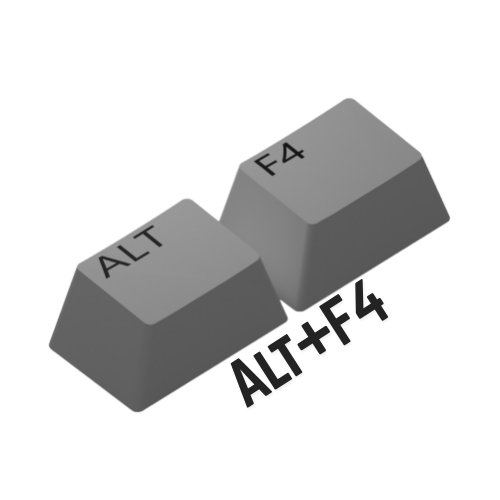
\includegraphics[width=0.5\textwidth]{../Immagini/logoNome.png}
        \end{center}
        \vfill
        \begin{center}
            \begin{spacing}{2} 
                \textbf{\Huge Titolo documento} \\
                \Large \today
            \end{spacing}
        \end{center}
        \vfill
    \end{titlepage}

    \tableofcontents
    
    \newpage

    \begin{table}[!h]
        \centering
        \caption*{\textbf{\Huge Registro Modifiche}}
        \begin{tabular}{| c | c | c | c |}
            \hline
            \textbf{\large Versione} & \textbf{\large Data} & \textbf{\large Autore/i} & \textbf{\large Descrizione} \\ 
            \hline \hline
            v0.1 & Data & Nome & Descrizione modifica \\
            \hline 
        \end{tabular}
    \end{table}
    \newpage

    % INIZIO CONTENUTO

    \section{Esempio sezione principle}
    Testo sezione principale.

    \subsection{Esempio sezione secondaria}
    Testo sezione secondaria.

    %Esempio elenco puntato
    \begin{itemize}
        \item Primo elemento
        \item Secondo elemento 
    \end{itemize}

    %Esempio elenco numerato
    \begin{enumerate}
        \item Primo elemento
        \item Secondo elemento
    \end{enumerate}
    
    \textit{Questo è un testo in corsivo}.
    
    \glossario{Termine di glossario}

\end{document}